\documentclass[a4paper,12pt]{article} 
\usepackage[utf8]{inputenc}
\usepackage[english, russian]{babel}
\usepackage{amsmath, soulutf8, nopageno} % "nopageno" removes page numeration
\usepackage{graphicx, caption, wrapfig} % For image
\usepackage[left=10mm, top=20mm, right=10mm, bottom=20mm]{geometry}

\begin{document}
\setcounter{equation}{34}
\noindent
124 \hfill \textbf{Уравнение первого порядка} \hfill [ГЛ. III] \\

Уравнение (34') ставит в соответствие каждой точке (x, y) одно или несколько значенией $\dfrac{dy}{dx}$, определяющих поле направлений данного семейства. Мы можем положить $x = x_1, y = y_1$; направление поля для изогональных траекторий связано с направлением поля для данного семейства соотношением (32), откуда. разрешая относительно $\dfrac{dy}{dx}$, имеем: 
$$
	\frac{dy}{dx} = \dfrac{ \dfrac{dy_1}{dx_1}-k }{ k\cdot\dfrac{dy_1}{dx_1}+1 }.
$$
Вставляя это выражение в уравнение (34'), с заменой в нем x, y соответственно на $x_1, y_1$, получаем уравнение поля для семейства изогональных траекторий, т. е. их диференциальное уравнение: 
\begin{equation}
	\Phi_1\Bigg(x_1, y_1, \dfrac{ \dfrac{dy_1}{dx_1}-k }{ k\cdot\dfrac{dy_1}{dx_1}+1 }\Bigg)=0.
\end{equation}
В случае ортогональных траекторий $\dfrac{dy}{dx}$ и $\dfrac{dy_1}{dx_1}$ связаны отношением: 
$$
	\frac{dy}{dx} = -\dfrac{ 1 }{ \dfrac{dy_1}{dx_1}},
$$
откуда диференциальное уравнение для ортогональных траекторий

\begin{equation} 
	\Phi_1\Bigg(x_1, y_1, -\dfrac{ 1 }{ \dfrac{dy_1}{dx_1} }\Bigg)=0.\tag{35'}
\end{equation}

\so{Примечание}. В дальнейшем мы будем отбрасывать индексы и обозначать координаты точки траектории также через x, y там, где это не может вызвать путаницы.

\textit{Пример 24}. Найти изогональные траектории пучка прямых с центром в начале координат: $y=ax$. Пусть угол пересечения $x \neq \dfrac{\pi}{2}, \tg{a}=k$. Имеем:
$$
	\dfrac{dy}{dx}=a, \ \ \dfrac{\dfrac{dy_1}{dx_1}-\dfrac{dy}{dx}}{1+\dfrac{dy_1}{dx_1}\cdot\dfrac{dy}{dx}}=k,
$$
заменяя $\dfrac{dy}{dx}$ его значением $a$, которое в силу уравнения семейства равно $\dfrac{y_1}{x_1}$, получаем (опуская индексы):
$$
	\dfrac{\dfrac{dy}{dx}-\dfrac{y}{x}}{1+\dfrac{y}{x}\cdot\dfrac{dy}{dx}}=k,
$$
или
$$
	\dfrac{dy}{dx}=\dfrac{y+kx}{x-ky}.
$$
\newpage
 \hfill \textbf{Уравнение первого порядка} \hfill 125 \\

Это уравнение однородное, но оно проще интегрируется при помощи интегрирующего множителя:
$$
xdy-ydx=k(xdx+ydy),
$$
$$
	\frac{xdx+ydy}{x^2+y^2}=\frac{1}{k}\frac{xdy-ydx}{x^2+y^2},
$$
откуда
$$
	\frac{1}{2}\ln{(x^2+y^2)}=\frac{1}{k}\arctg{\dfrac{x}{y}}+\ln{C},
$$
или
$$
	\sqrt{x^2+y^2}=Ce^{\frac{1}{k}\arctg{\frac{y}{x}}}
$$
или, наконец, в полярных координатах $r=Ce^\frac{\varphi}{k}$ (семейство логарифмических спиралей).

Если $a=\dfrac{\pi}{2}$, то имеем:
$$
	\dfrac{dy_1}{dx_1}=-\dfrac{1}{\dfrac{dy}{dx}}=-\dfrac{1}{a}=\dfrac{1}{\dfrac{y_1}{x_1}}
$$
или
$$
	x_1dx_1+y_1dy_1=0
$$
или $x_1^2+y_1^2=C$ \--- семейство окружностей. 

\textit{Пример 25}. Имеем семейство софокусных эллипсов с фокусаи в точках: $x=\pm1, y=0:$
$$
	\dfrac{x^2}{1+\lambda}+\dfrac{y^2}{\lambda}=1 \ \ \ \ (\lambda > 0).
$$
Их диференциальное уравнение будет (гл. 1, \S 1, 4):

\begin{wrapfigure}{r}{0.5\textwidth}
	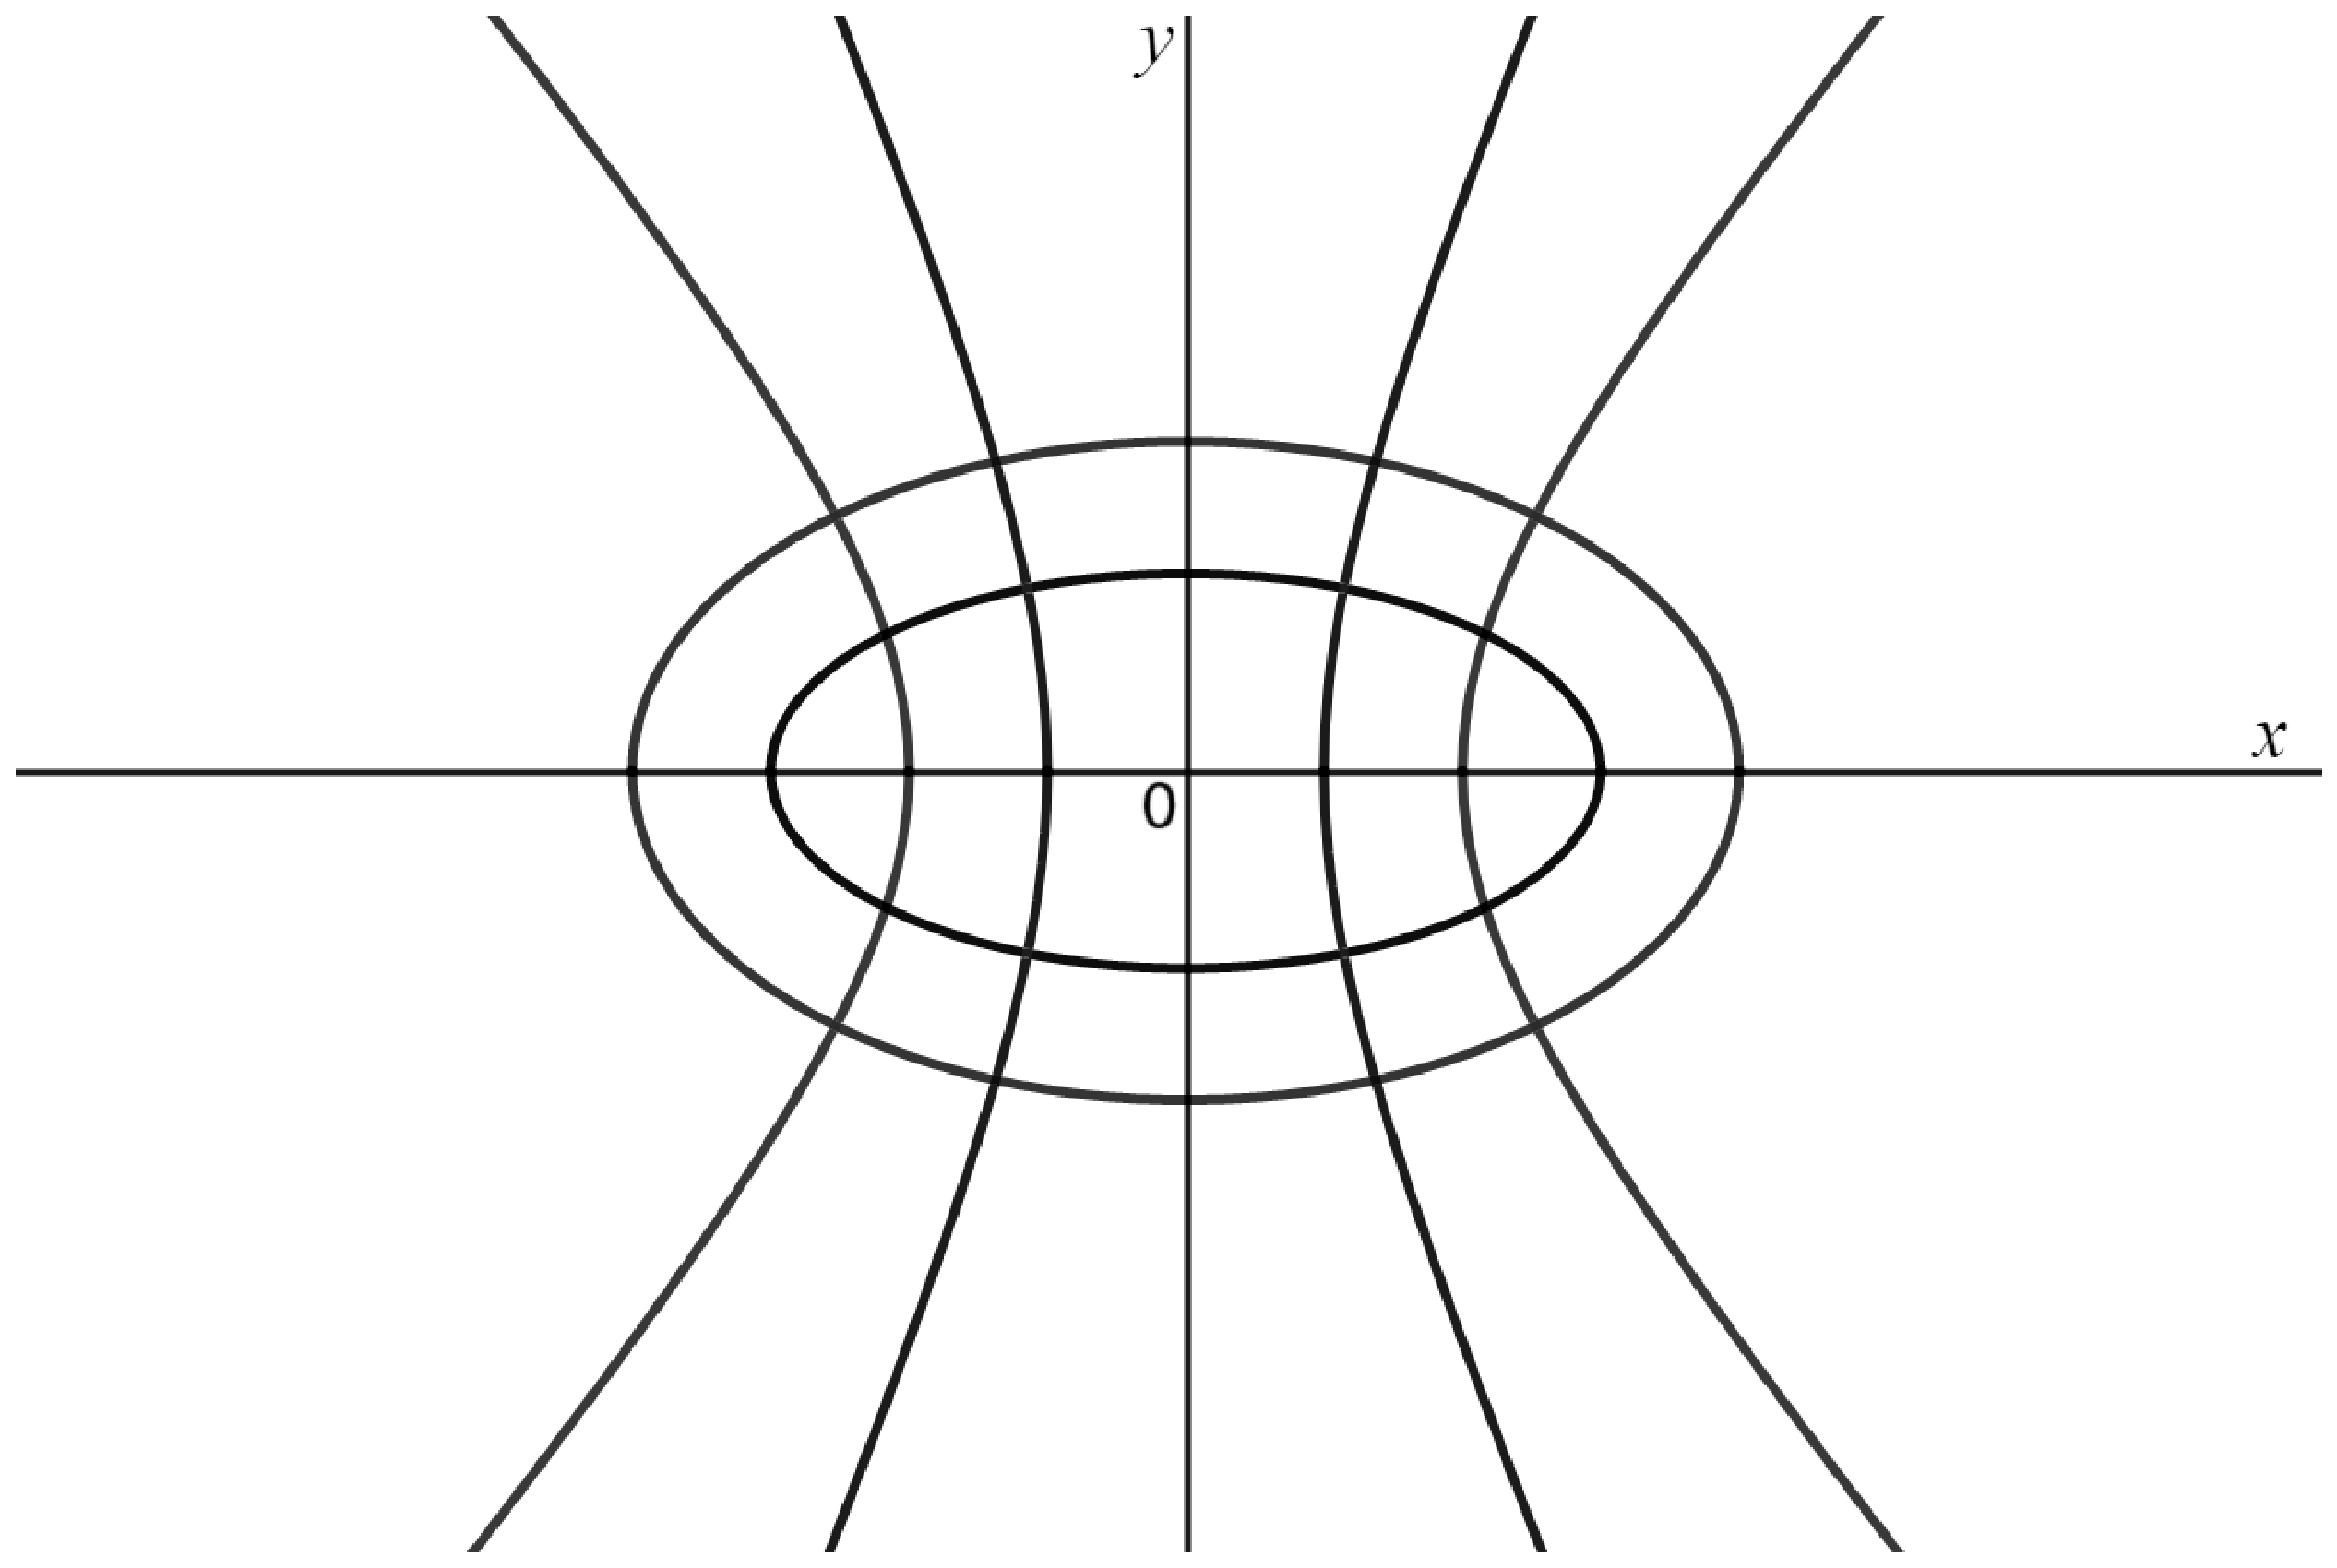
\includegraphics[width=\linewidth]{desmos-graph.eps}
	\caption * {Черт. 23.} % * removes standard numeration (package caption)
\end{wrapfigure}
$$
	(xy'-x)(x+yy')=y',
$$
или
$$
	xyy'^2+(x^2-y^2-1)y'-xy=0.
$$

Чтобы получить диференциальное уравнение ортогональных траекторий, достаточно заменить в этом уравнении $y'$ на $-\dfrac{1}{y'}$; получаем:
$$
	\dfrac{xy}{y'^2}-\dfrac{(x^2-y^2-1)}{y'}-xy=0,
$$
или
$$
	xyy'^2+(x^2-y^2-1)y'-xy=0,
$$\\
т. е. то же уравнение. Дело объясняется тем, что данное уравнение \--- второй степени относительно y; через каждую точку проходят две кри-
\end{document}

